\documentclass[10pt, conference]{IEEEtran}
\IEEEoverridecommandlockouts

\usepackage{cite}
\usepackage[pdftex]{graphicx}
\graphicspath{{figure/}}
\usepackage[cmex10]{amsmath}
\interdisplaylinepenalty=2500
%\usepackage{algorithmic}
%\usepackage{array}
\usepackage[caption=false,font=footnotesize]{subfig}
%\usepackage{fixltx2e}
\usepackage{stfloats}
\fnbelowfloat
\usepackage{url}
\usepackage{multirow}
\usepackage{booktabs}

% correct bad hyphenation here
\hyphenation{op-tical net-works semi-conduc-tor}

\begin{document}
\title{Parallel Hardware Merge Sorter}


\author{
  \IEEEauthorblockN{
    Wei~Song\IEEEauthorrefmark{1}\IEEEauthorrefmark{2},
    Dirk~Koch\IEEEauthorrefmark{2},
    Mikel~Luj\'{a}n\IEEEauthorrefmark{2}\thanks{Dr Luj{\'a}n is funded by a Royal Society University Research Fellowship.},
    and~Jim~Garside\IEEEauthorrefmark{2}}
  \IEEEauthorblockA{\IEEEauthorrefmark{1}Computer Laboratory, University of Cambridge, Cambridge CB3 0FD, UK}
  \IEEEauthorblockA{\IEEEauthorrefmark{2}School of Computer Science, University of Manchester, Manchester M13 9PL, UK}
  \IEEEauthorblockA{ws327@cam.ac.uk; \{dirk.koch; mikel.lujan; james.garside\}@manchester.ac.uk}
}

\maketitle

\begin{abstract}

Sorting has tremendous usage in the applications that handle massive amount of data.
Existing techniques accelerate sorting using multiprocessors or GPGPUs where a data set is partitioned into disjunctive subsets to allow multiple sorting threads working in parallel.
Hardware sorters implemented in FPGAs have the potential of providing high-speed and low-energy solutions
but the partition algorithms used in software systems are so data dependent that they cannot be easily adopted.
The speed of most current sequential sorters still hangs around 1~number/cycle.
Recently a new hardware merge sorter broke this speed limit by merging a large number of sorted sequences at a speed proportional to the number of sequences.
This paper significantly improves its area and speed scalability by allowing stalls and variable sorting rate.
A 32-port parallel merge-tree that merges 32 sequences is implemented in a Virtex-7 FPGA.
It merges sequences at an average rate of 31.05 number/cycle and reduces the total sorting time by 160 times compared with traditional sequential sorters.

\end{abstract}

\begin{IEEEkeywords}
Merge sort, sorting network, parallel sorting, FPGA.
\end{IEEEkeywords}


\section{Introduction}

As a key part in numerous computer algorithms, sorting has tremendous usage in many applications.
It is an important step of the reduce function used in the MapReduce programming model~\cite{Dean2008},
which is the \emph{de facto} distributed model for processing massive data sets on server clusters.
For relational databases, join is one of the fundamental query operations.
As one of the most utilized join implementation, sort-merge join~\cite{Mishra1992} combines two tables by firstly sorting their keys.
Low latency sorting is also required in some scientific computing~\cite{Farmahini-Farahani2011}.
In fact, sorting is so important that various sorting benchmarks~\cite{SortBenchmark} have been defined to regularly rank the top sorters ever built.


The methods of accelerating sorters have been researched for several decades using various devices,
such as parallel computers~\cite{Cole1988}, dedicated application specific integrated circuits (ASICs)~\cite{Arisland1984, Tsuda1987, Farmahini-Farahani2013},
field programmable gate arrays (FPGAs)~\cite{Marcelino2009, Koch2011, Mueller2012, Casper2014},
multiprocessors~\cite{Gedik2007,Chhugani2008,Odeh2012} and recently general-purpose graphic processing units (GPGPUs)~\cite{Govindaraju2006, Satish2009}.
Sorting becomes increasingly important these days due to the fast growing amount of data in certain applications,
where database is one of the most active areas~\cite{Mueller2012, Casper2014}.


The state-of-the-art research on sorter accelerating concentrates on software sorting algorithms~\cite{SortBenchmark}.
A large data set can be divided into disjunctive subsets~\cite{Odeh2012}; therefore, subsets can be sorted by multiple threads in parallel.
Since this partition procedure is highly data dependent, it is not directly applicable for hardware sorters,
although hardware sorters have the potential of providing high-speed and low-energy sorting solutions.
Up to now, there is no easy way of making hardware sorters run in parallel. % for a decent amount of data.


Existing hardware sorters are either parallel or sequential sorters.
Parallel sorters, such as sorting networks~\cite{Batcher1968}, 
can sort up to only hundreds of numbers~\cite{Farmahini-Farahani2013} due to the limited number of I/O ports.
As an alternative, sequential sorters~\cite{Bitton1984} can sort a large data set but at a low sorting rate of usually 1~number/cycle.
Such low speed significantly limits the benefit of using FPGAs as sorting accelerators. %, not to mention the frequency mismatch between processors and FPGAs.
Without a method to sort a large data set in parallel, hardware sorters are actually slower than software sorters running on processors considering the gap in clock frequencies.

This paper proposes a parallel merge-tree which merges multiple sorted data sequences at a speed proportional to the number of sequences.
It has three major advantages over sequential sorters:
\begin{itemize}
\item The sorting rate is significantly increased from 1 number/cycle up to 1 number/cycle/sequence.
\item Merging more than 2 sequences significantly reduces the number of passes (runs) to sort a large data set.
\item The parallel merge-tree merges data in a streamed fashion.
The size of the sorted data is not constrained by the available on-FPGA memory, which is used only as communication buffers for the main memory.
\end{itemize} 
A 32-port parallel merge-tree is implemented in a Xilinx Virtex-7 XC7VX485T FPGA~\cite{virtex72015}.
It merges 32 sequences at a rate up to 32 number/cycle.
When sorting a large data set, using this 32-port parallel merge-tree reduces the total sorting time by nearly 160 times compared with sequential sorters.

\section{Existing Sorters}

The proposed parallel merge-tree is developed from existing sorters and can be used along with other designs to form large sorting systems.
The related hardware and software sorters are briefly reviewed to provide a limited background introduction.
As a sorter can sort numbers in either descending or ascending order, all sorters described in this paper use the descending order to avoid ambiguity.


A large scale sorting system is normally composed of tens to thousands of server nodes~\cite{SortBenchmark}.
The input data are divided into disjunctive subsets using foreknown statistics or an initial sampling~\cite{Graves2013, Conley2014, Wang2015}.
These subsets are sorted by parallel servers simultaneously and then merged into a final sorted sequence.
%The tasks of 
Subset partition and workload balancing among servers are fulfilled by software~\cite{Graves2013, Wang2015} due to their data dependence and irregular control patterns.
The actual sorting acceleration happens in the individual sorting server which sorts a subset or merges the final sequence.
Current servers use off-the-shelf solutions such as high performance multiprocessors~\cite{Graves2013, Conley2014, Wang2015} or GPGPUs~\cite{Govindaraju2006,Satish2009}.
The proposed parallel merge-tree can be dynamically reconfigured to an FPGA as a sorting accelerator cooperating with a server,
which is potentially more energy and cost efficient than sorting in processors.
Although this configuration is rarely used in present datacenters, it is likely to become popular with the availability of high-performance embedded cores in future large capacity FPGAs (e.g. Xilinx UltraScale+ or Altera Stratix 10).
%although the research of using FPGAs as such application specific accelerators is in its early stage.


Servers choose different sorting algorithms according to statistics and available resources.
To reduce sorting time, it is important to sort in parallel but not all sorting algorithms can be parallelized easily.
\emph{Merge sort} and \emph{radix sort} are two extensively utilized algorithms which are both parallelizable but with very different nature.
Merge sort is a comparison sorting algorithm which merges normally two sorted sequences into one.
An unsorted data set can be sorted by recursively applying merge sort in multiple passes (also called runs in related literature).
The single-thread time complexity of sorting $N$ numbers is $O(N \log N)$.
Radix sort is a distribution sorting algorithm which sorts numbers by processing individual digits.
The sorting time is therefore proportional to the bit-width of numbers.
The single-thread time complexity of sorting $N$ numbers of $k$ bits is $O(N \cdot k)$.
Generally speaking, merge sort is faster than radix sort when sorting a bounded size of wide numbers ($k > \log N$),
which could be the case for a server that sorts only a subset of the whole data.
Merge sort is the target sorting algorithm researched in this paper.


Merge sort can be parallelized for running on multi-thread processors~\cite{Satish2009, Odeh2012}.
The two input sequences are partitioned into an arbitrary number of disjunctive and equal-sized segments in linear time~\cite{Odeh2012}.
Then each segment is merged on a different thread.
For a server with $p$ hardware threads, the time complexity of a parallel merger is $O(N/p \cdot \log N + \log p \cdot \log N)$~\cite{Odeh2012},
providing a speed up slightly less than $p$.


Hardware sorters are circuit implementations of certain sorting algorithms using ASICs or FPGAs.
Most hardware sorters can be classified into either parallel sorters or sequential sorters.
The most used parallel sorters are Bitonic and odd-even sorting networks~\cite{Batcher1968}.
Both of them sort $N$ numbers in $O(\log^2N)$ cycles.
However, the size of a sortable sequence is constricted by the number of I/O ports,
which is limited to hundreds~\cite{Farmahini-Farahani2013} in current VLSI technology.
Sequential sorters are the actual sorters able to sort large scale data sets.


Most sequential sorters implement single-thread sorting algorithms in hardware and run in a streamed fashion.
The sorted data is normally produced at a constant rate of 1 number/cycle,
such as the parallel shift sort (insertion sort)~\cite{Arisland1984}, the up/down sorter (heap sort)~\cite{Moore1995} and the FPGAsort (merge sort)~\cite{Koch2011}.
In all sequential sorters, FPGAsort is currently the most area efficient sorter thanks to its smart use of on-chip memory.
The size of a sortable sequence is usually constricted by the accessible storage space (on-chip and off-chip), which can be huge.
Compared with hardware parallel sorters, sequential sorters can sort a large scale data set but at a very low speed.


Numerous attempts have been made to parallelize sequential sorters.
For hardware merge sorters, both the early parallel merge module~\cite{Liu1989} and the recent high bandwidth sort merge unit~\cite{Casper2014}
use a tree of merge units to merge more than 2 input sequences simultaneously.
However, both sorters choose to enforce non-stall flow control for a constant sorting rate.
As a result, all merge units in the tree must run at the maximum rate,
which significantly increases area and the required memory bandwidth.
Such sorters are not very scalable.
The more recent high bandwidth sort merge unit is able to merge up to 8 sequences
but requires a staggering memory bandwidth of more than 6 times of the sorting rate~\cite{Casper2014}.


The parallel merge-tree proposed in this paper also uses a tree of merge units.
The decisive difference with the aforementioned two is to allow stalls and variable sorting rate in order to pursue a high accumulated sorting speed.
In this way, non-root merge units run at lower sorting rates than the root one and consume less area.
More importantly, the required memory bandwidth is reduced to just the maximum sorting rate.
Compared with the software parallel merger~\cite{Odeh2012}, merging more than 2 sequences in each pass provides extra speed up due to the reduced number of passes. 

\section{Multirate Merging}

A traditional hardware merge sorter, such as the FPGAsort~\cite{Koch2011}, produces sorted data at a speed of 1 number/cycle.
A multirate merger (MM) is able to merge two sorted sequences at a speed much faster than 1 number/cycle.

\subsection{Comparator units}

Various comparator units~\cite{Farmahini-Farahani2013} perform the basic comparing and exchanging operations needed by the sorters in this paper.
A full compare-and-exchange (CAE) unit compares 2 input numbers and outputs both of them in order.
\figurename~\ref{fig_cae} depicts the implementation (left) of a CAE unit and its symbol (right).
When only 1 output is needed (assuming the larger one),
a CAE unit is reduced to a compare-and-select (CAS) unit~\cite{Farmahini-Farahani2013} as shown in \figurename~\ref{fig_cas}.
For some sorters, the selection result of a CAS unit is used by further circuitry.
Such a CAS unit with a selection feedback signal \emph{s} is depicted in \figurename~\ref{fig_cass}.

\begin{figure}[bt]
\centering{
\subfloat[]{\includegraphics[width=0.15\textwidth]{figure/cae_circuit} \quad \includegraphics[width=0.13\textwidth]{figure/cae_symbol}\label{fig_cae}}\\
\subfloat[]{\includegraphics[width=0.15\textwidth]{figure/cas_circuit} \quad \includegraphics[width=0.13\textwidth]{figure/cas_symbol}\label{fig_cas}}\\
\subfloat[]{\includegraphics[width=0.15\textwidth]{figure/cass_circuit} \quad \includegraphics[width=0.13\textwidth]{figure/cass_symbol}\label{fig_cass}}
}
\caption{Implementations and symbols of comparator units: (a) Compare-and-exchange (CAE), (b) compare-and-select (CAS), and (c) CAS with a selection feedback.}\label{fig_cunit}
\end{figure}

\subsection{Parallelization}

The structure of a FIFO merge sorter (unoptimized FPGASort)~\cite{Marcelino2008, Koch2011} is illustrated in \figurename~\ref{fig_fifomerge}.
It comprises three parts: two FIFOs to store the input sequences
and a CAS unit to output the largest number remaining in the two FIFOs.

\begin{figure}[bt]
\centering{
\includegraphics[width=0.18\textwidth]{figure/fifomerge}
}
\caption{A FIFO merge sorter.}\label{fig_fifomerge}
\end{figure}

A multirate merger is an expanded FIFO merge sorter which shares the same overall structure but with more complicated components in each part.
An abstract view of a multirate merger which provides $P$ sorted number per cycle, MM($P$), is depicted in \figurename~\ref{fig_pmerger_concept}.
It also needs two FIFOs to store the input sequences but the CAS unit is replaced with a parallel sorter
which extracts and sorts the largest $P$ numbers remaining in the two FIFOs.
Since these numbers may come from the same FIFO due to imbalanced distribution,
the parallel sorter needs to pick them from a total of $2P$ numbers.

\begin{figure}[bt]
\centering{
\includegraphics[width=0.22\textwidth]{figure/pmerger_concept}
}
\caption{MM($P$), a $P$-port multirate merger (abstract view).}\label{fig_pmerger_concept}
\end{figure}

For the multirate merger to work, two issues must be resolved:

\begin{itemize}
\item The unchosen numbers must be retained in FIFOs for the next cycle.
Therefore, the selection of the largest $P$ numbers must be finished in one cycle to avoid extra feedback delay.
\item The FIFOs have a variable data rate between 0 to $P$~number/cycle,
which is not directly supported by normal FIFO designs.
\end{itemize}

\subsection{Single-cycle selection}

The solution for the single cycle selection is to use a Bitonic partial merger,
which is a part of a Bitonic sorting network and has been analysed recently by Farmahini-Farahani~\cite{Farmahini-Farahani2013}.

An 8-to-4 Bitonic partial merger is shown in \figurename~\ref{fig_bpmerger}.
It reads numbers from two sorted sequences $[I_3 \cdots I_0]$ and $[I_7 \cdots I_4]$,
picks the largest 4 numbers, and shuffles them into a sorted sequence $[O_3 \cdots O_0]$.
The merger is fully pipelined into 3 stages and the selection process occurs on the first stage.

\begin{figure}[bt]
\centering{
\includegraphics[width=0.22\textwidth]{figure/bpm8t4}
}
\caption{An 8-to-4 Bitonic partial merger.}\label{fig_bpmerger}
\end{figure}

For an MM($P$), a $2P$-to-$P$ Bitonic partial merger is used to choose the largest $P$ numbers
remaining in the two FIFOs and sort them in a pipelined way.
The selection result is available from the first pipeline stage;
therefore, it can be used to retain the unselected data in the same cycle.
Furthermore, Bitonic sorting networks are known to be area efficient.
Since the Bitonic partial merger is a part of the sorting network, it is also area efficient and scalable.

\subsection{Area-efficient FIFO implementation}\label{sec_fifo_imp}

The FIFOs are shallow but have a variable output rate from 0 to $P$ number/cycle depending on the selection result.
It is not easy to use dual-port memory blocks due to this variable rate and a full register-based design is area consuming.
The most area-efficient solution so far is to divide a wide FIFO into $P$ parallel narrow FIFOs, each of which is only 1 number wide.
Since now the output rate of each narrow FIFO is 0 or 1 number/cycle, it can be implemented in special shift register look-up tables (SRLs) which are abundant in Virtex FPGAs~\cite{virtex7CLB2014}. 
Every SRL can be used as a 16-bit shift register.

The detailed implementation is demonstrated in \figurename~\ref{fig_pmfifo}. It has $P$ narrow FIFOs implemented in SRLs.
Two crossbars connect FIFOs to the input sequence (\emph{I}) and the Bitonic partial merger (\emph{D}).
The selection result, denoted as \emph{s}, is fed back to individual FIFOs to identify whether there is shift occurring in the current cycle.
Also under the control of the selection result, the output crossbar ensures the FIFO that has the largest remaining number is always connected to \emph{D$_0$}.

\begin{figure}[bt]
\centering{
\includegraphics[width=0.38\textwidth]{figure/pmfifo}
}
\caption{An FIFO for multirate mergers.}\label{fig_pmfifo}
\end{figure}

The output crossbar is implemented as an array of barrel shifters~\cite{Gigliotti2004} controlled by signal \emph{offset}. Depending on the value of \emph{offset}:
\begin{equation}
[D_{P-1} \cdots D_0] = [F_{\text{offset}-1} \cdots F_{0}, F_{P-1} \cdots F_{\text{offset}} ]
\end{equation}
The input sequence is sorted in descending order.
Initially, the largest number is stored in $F_0$ and connected to $D_0$ (\emph{offset} = 0).
To ensure that $D_0$ always has the largest number and $D$ is in descending order,
\emph{offset} tracks the selection result closely:
\begin{equation}
  \text{\emph{offset'}} = \text{\emph{offset}} + \text{\emph{rate}}
\end{equation}
where \emph{offset'} is the next cycle's value of \emph{offset} and \emph{rate} is the amount of numbers shifted in the current cycle, accumulated from the selection result $s$:
\begin{equation}
  \text{\emph{rate}} = \sum\limits_{i=0}^{P-1} s_i
\end{equation}

Fortunately the conversion from $s$ to \emph{rate} does not really need an accumulator since $D$ is sorted.
For any $D_i \in D$, if $D_i$ is selected, $[s_i \cdots s_0]$ must be all ones
because any number in $[D_{i-1} \cdots D_0]$ is larger than $D_i$ and must be selected as well.
As a result, the conversion from $s$ to \emph{rate} can be summarized in Table~\ref{tab_conv}.
The corresponding implementation of a rate converter is depicted in \figurename~\ref{fig_rate_conv}.
The first column of AND/INV gates translate $s$ into $m$ which is the one-hot format of \emph{rate}.
Then a one-hot to binary (OH2Int) circuit provides the \emph{rate}.

\begin{table}
\caption{Converting $s$ to \emph{rate}}\label{tab_conv}
\centering
\begin{tabular}{cc}
\toprule
$[s_{P - 1} \cdots {s_0}]$ & \emph{rate} \\
\midrule
 $\forall i, {s_i} = 0$ & 0 \\
 $(\forall i < m, {s_i} = 1) \wedge (\forall i \ge m, {s_i} = 0)$ & $m$ \\
 $\forall i, {s_i} = 1$  & $P$ \\
\bottomrule
\end{tabular}
\end{table}

\begin{figure}[bt]
\centering{
\includegraphics[width=0.22\textwidth]{figure/rate_conv}
}
\caption{A rate converter for MM(4).}\label{fig_rate_conv}
\end{figure}

The FIFO inputs work in a similar way with outputs. The data rate of the input sequence is $P/2$ number/cycle.
The input crossbar (another array of barrel shifters)\footnote{A crossbar is needed when the length of input sequences is not always times of $P/2$;
otherwise a de-multiplexer is enough.} ensures the input sequence is stored in the correct narrow FIFOs in a round-robin style.
The \emph{offset} signal for the input crossbar is controlled by the \emph{full} signal of the FIFO inputs.

\subsection{Multirate merger}\label{sec_pmerger_imp}

Putting all components together, \figurename~\ref{fig_pmerger_imp} reveals the implementation of an MM($P$).
Two sorted input sequences ($I_0$ and $I_1$) are stored in two parallel FIFOs.
The outputs of FIFOs, denoting the largest $P$ numbers of each FIFO, are fed to a $2P$-to-$P$ Bitonic partial merger,
which selects the largest half and sorts them into the output sequence $O$ at a rate of $P$~number/cycle. 

\begin{figure}[bt]
\centering{
\includegraphics[width=0.48\textwidth]{figure/pmerger}
}
\caption{MM($P$), a $P$-port multirate merger (implementation).}\label{fig_pmerger_imp}
\end{figure}

The selection result ($s$) is fed to the two FIFOs slightly differently. For FIFO$_0$, the selection result is inverted:
\begin{equation}
s_{\text{FIFO}_0}(i) = \bar{s_i}
\end{equation}
When $s_i$ is 0, $D_0(i)$ is selected rather than $D_1(P-i)$, therefore $s_{\text{FIFO}_0}(i)$ should be 1.
As for FIFO$_1$, the selection result is flipped due to the flipped connection to the Bitonic merger:
\begin{equation}
s_{\text{FIFO}_1}(i) =s_{P-i}
\end{equation}
When $s_{P-i}$ is 1, $D_1(i)$ is selected rather than $D_0(P-i)$, therefore $s_{\text{FIFO}_1}(i)$ should be 1.

The critical path of a multirate merger starts from the FIFO outputs,
traverses through the first stage of the Bitonic merger, the selection feedback and finally to the full signal of the FIFO outputs.
Since both the FIFO and the Bitonic merger is fully parallelized, the output crossbar is the only component affected
by the number of ports\footnote{For simplicity, we ignore the timing effect caused by increased area for this analysis.}.
Normally the latency of a crossbar is roughly linear with $\log P$.
The speed scalability of multirate mergers is expected to be $\log P$ as well.

The area of a multirate merger is dominated by the narrow FIFOs and the Bitonic partial merger.
The area of FIFOs is proportional to $P$ while the area of the Bitonic partial merger is linear with $P \log P$~\cite{Farmahini-Farahani2013}.
As a result, the area complexity of an MM($P$) is $O(P \log P)$.

\subsection{Rate mismatch}\label{sec_pmerge_mismatch}

The FIFO input data rate is set to $P/2$ number/cycle for an MM($P$).
When numbers are perfectly balanced between sequences, the output rate is $P$ number/cycle.
The $P/2$ number/cycle input rate is enough to maintain the output rate.
When numbers are not balanced, the Bitonic partial merger may consecutively choose numbers from one sequence at a rate larger than $P/2$ number/cycle,
which causes rate mismatch in both FIFOs. If one FIFO is eventually empty, the multirate merger is stalled waiting the empty FIFO to be refilled.

There are two ways to handle this issue:
One is to increase the input rate to $P$ number/cycle in order to avoid stalls,
the other one is to accept stalls with flexible control logic.
Rather than increasing the input rate as the high bandwidth sort merge unit~\cite{Casper2014} does,
the multirate merger adopts the latter solution
because the accummulated input rate of the former solution is unsustainable when merging mutiple sequences.
More insights will be provided in Section~\ref{sec_pmt_mismatch} where the parallel merge-tree has been introduced.

\subsection{Optimization for skewed data}\label{sec_skew_opt}

When a data set is skewed, the probability of duplicated numbers increases.
Since CAS units (shown in \figurename~\ref{fig_cunit}) choose a fixed input when the two inputs are equal,
duplicated numbers cause stalls in a way similar to the imbalanced data distribution.

An easy way to resolve this issue is to ask the CAS units in the first stage of the Bitonic partial merger to choose different inputs.
The rule is simple: For CAS$_i$ that compares $D_0(i)$ and $D_1(P-i)$,
when the two numbers are equal, CAS$_i$ chooses $D_0(i)$ if $i < P/2$, otherwise $D_1(P-i)$.
As a result, instead of causing rate mismatch between FIFOs, duplicated numbers provide opportunities to re-balance FIFOs.
Extremely skewed data actually results in lower stall rates than randomly and uniformly distributed data, as shown in Section~\ref{sec_skewed_data}.

\section{Parallel Merge-Tree}

Using multiple levels of multirate mergers, a parallel merge-tree (PMT) is able to merge multiple sorted sequences simultaneously.

\subsection{Merging multiple sequences}

An 8-port parallel merge-tree is shown in \figurename~\ref{fig_pmtree}.
When the number of levels $L = \log P$, $P$ input sequences are merged,
the input rate for each input sequence is only 1 number/cycle,
and the output rate is up to $P$ number/cycle.

\begin{figure}[bt]
\centering{
\includegraphics[width=0.36\textwidth]{figure/pmtree}
}
\caption{PMT(8), an $8$-port parallel merge-tree.}\label{fig_pmtree}
\end{figure}

Since the area complexity of MM($P$) is $P \log P$,  the area complexity of a PMT(P):

\begin{equation}\label{eqn_pmt_area}
\sum\limits_{i = 1}^{\log P} (O(2^i \cdot \log 2^i) \cdot P/2^i) = \sum\limits_{i = 1}^{\log P} iP = O(P\log ^2P)
\end{equation}

Two important observations are revealed here:
The accumulated input rate (requirement for memory bandwidth) is equal with the maximum output rate;
and the area of parallel merge-trees is scalable to $O(P\log ^2P)$.

\subsection{Revisiting rate mismatch}\label{sec_pmt_mismatch}

Similar to multirate mergers, a parallel merge-tree has the rate mismatch issue.
When numbers are perfectly balanced in all input sequences, the output rate is stable at $P$ number/cycle.
However, when numbers are distributed unevenly, the output rate is reduced due to stalls.
In the worst case, when numbers are forced to be read sequentially from one sequence to another, the average output rate is dropped to 1 number/cycle.
The proposed parallel merge-tree is only suitable for evenly or randomly distributed data sets.
A pre-sorted data set needs to be randomly reshuffled before sent to a parallel merge-tree.

For randomly distributed data sets, results in Section~\ref{sec_stall_rate_ana} will demonstrate
that the stall rate can be reduced to a negligible level by moderately increasing the depth of FIFOs.

As discussed in Section~\ref{sec_pmerge_mismatch}, a solution to avoid stalls is to increase the input rate of multirate mergers,
which is used in the high bandwidth sort merge unit~\cite{Casper2014}.
In this case, all the multirate mergers in \figurename~\ref{fig_pmtree} are replaced with MM(8)s.
This solution has two outstanding drawbacks.

One is the increased area. For a $P$-port merge-tree, the number of mergers needed is $P-1$.
Therefore, the area complexity increases to:
\begin{equation}
O(P \log P) \cdot (P-1) = O(P^2 \log P)
\end{equation}
Compared with Equation~\ref{eqn_pmt_area}, the area is increased by $P / \log P$ times.

The other drawback, which is even worse, is the significantly increased input data rate.
Since the data rate of all input sequences is increased to the maximum output rate,
the accumulated input rates of a $P$-port tree is increased to $P^2$ number/cycle, $P$ times of the output rate.
As reported in the high bandwidth sort merge unit~\cite{Casper2014}, to merge 8 sequences using a 2-level tree,
the accumulated memory bandwidth is 6 times of the sorting rate. Clearly this method is not scalable.

We believe allowing mergers to stall is the right choice.
The results in this paper demonstrate that the achievable stall rate for most data sets is very small.
The benefits of reduced area and memory bandwidth outweigh the slightly reduced sorting rate,
and the achievable sorting rate is significantly higher than using the high bandwidth sort merge units.

\section{Performance Evaluation}

Several parallel merge-trees have been implemented on a Virtex-7 XC7VX485T FPGA~\cite{virtex72015}.
Rather than sorting numbers, practical sorting systems sort records.
A record comprises of a key field and an information field.
The key field is used in sorting the records while the attached information to each key represents the real data stored in the record.
In this paper, all implementations sort records of 64 bits, where both the key field and the information field are 32 bits wide.
The stall rate evaluation is based on cycle accurate simulation
while the scalability analysis reports post-route results and experiments running on the FPGA.
In order to evaluate the pure sorting hardware, we used test pattern generators and a result checker instead of an I/O system.

\subsection{Stall rate evaluation}\label{sec_stall_rate_ana}

A multirate merger stalls when one of its FIFOs becomes empty due to imbalanced data distribution.
Increasing the depth of FIFOs reduces the probability of stalls.
To examine this stall reduction, a PMT(16) is used to merge 16 randomly and uniformly distributed sequences, each of which is 8K records long.
The depth of FIFOs is increased from 4 to 16.
The average stall rate is defined as the number of stalled cycles divided by the total number of cycles.
All test cases are run 10 times for averaging the result.
As shown in \figurename~\ref{fig_fifo_depth}, the average stall rate drops significantly at start with shallow FIFOs.
Such benefit becomes diminishing with longer FIFOs. 
Overall, the stall rate is reduced to a negligible level of 0.03 with a moderate depth of 16.

\begin{figure}[bt]
\centering{
\subfloat[]{\includegraphics[width=0.29\textwidth]{graph/fifo_depth}\label{fig_fifo_depth}}\\
\subfloat[]{\includegraphics[width=0.29\textwidth]{graph/pmt_area_fifo}\label{fig_pmt_area_fifo}}
}
\caption{(a) Stall rate and (b) area with different FIFO depths (a PMT(16) merging 16 sequences of 8K records each).}\label{fig_fifo_cfg}
\end{figure}

There is no observable area cost of increasing the FIFO depth up to 16 thanks to the implementation described in Section~\ref{sec_fifo_imp}.
\figurename~\ref{fig_pmt_area_fifo} reveals the utilization of FPGA resources, including look-up tables (LUTs), registers, and SRLs.
Although there is some variation on the total number of LUTs, the utilization of registers and SRLs is constant.
To take full advantage of the reduced stall rate, all the remaining implementations use FIFOs of 16 records deep.

The estimation of stall rate (data rate) is affected by the length of sequences.
\figurename~\ref{fig_seq_len} shows the normalized data rate (average rate divided by the maximum rate) of merging 16 sequences of different lengths.
The estimation error decreases with the increasing sequence length.
Interestingly, merging longer sequences results in slightly smaller data rate (higher stall rate).
We believe this is due to the higher probability of longer imbalanced segments.

\begin{figure}[bt]
\centering{
\includegraphics[width=0.29\textwidth]{graph/seq_len}
}
\caption{Normalized data rate of merging sequences with different lengths.}\label{fig_seq_len}
\end{figure}

According to the result, sequences of 8K records are chosen for other test cases
because they produce relatively accurate data rate estimation and are not too time-consuming to simulate (RTL simulation).

\subsection{Sorting skewed data}\label{sec_skewed_data}

\begin{table*}
\caption{Hardware Performance of Parallel Merge-Trees (FIFO Depth = 16)}\label{tab_pmt}
\centering
\begin{tabular}{ccccccccc}
\toprule
Ports     & Period & Frequency 
                             & Register       & LUT              & SRL    & Stall Rate
                                                                                    & Data Rate      & Data Rate\\
          & (ns)    & (MHz)  &                &                  &        &         & (Number/cycle) & (Gb/s)   \\
\midrule
2         & 4.02    & 248.5  & 328 (0.05\%)   & 853 (0.28\%)     & 132    & 1.75\%  & 1.97           & 31.3     \\
4         & 4.69    & 213.1  & 1534 (0.25\%)  & 4278 (1.41\%)    & 528    & 2.16\%  & 3.91           & 53.4     \\
8         & 6.12    & 163.3  & 5287 (0.87\%)  & 16016 (5.28\%)   & 1608   & 2.56\%  & 7.80           & 81.5     \\
16        & 7.50    & 133.4  & 16299 (2.68\%) & 47001 (15.48\%)  & 4238   & 2.74\%  & 15.56          & 132.9    \\
32        & 10.08   &  99.2  & 45445 (7.48\%) & 142179 (46.83\%) & 11379  & 2.98\%  & 31.05          & 197.1    \\
\bottomrule
\end{tabular}
\end{table*}

Practical data sets are usually skewed.
It is important for a sorter to handle skewed data efficiently.
An optimization was described in Section~\ref{sec_skew_opt}, which makes CAS units choosing different inputs to avoid the stalls caused by duplicated numbers.
Two PMT(16)s, an unoptimized one (original) and an optimized one, are injected with synthetic data sets generated~\cite{Gray1994} using 4 skewed distributions:
Exponential, Poisson, Pareto and Zipfian.
The results are shown in \figurename~\ref{fig_distribution}.
The optimized parallel merge-tree shows strong tolerance to skewed data while the original parallel merge-tree suffers seriously.
Interestingly, when the data is extremely skewed, such as $\lambda \ge 10$ for the exponential distribution and $\alpha \ge 10$ for the Pareto distribution,
the optimized parallel merge-tree appears to achieve the maximum rate.
We believe FIFOs are easily balanced when most of the numbers are equal.

\begin{figure}[bt]
\centering{
\subfloat[]{\includegraphics[width=0.22\textwidth]{graph/exp}\label{fig_exp}} \quad
\subfloat[]{\includegraphics[width=0.22\textwidth]{graph/poisson}\label{fig_poisson}} \\
\subfloat[]{\includegraphics[width=0.22\textwidth]{graph/pareto}\label{fig_pareto}} \quad
\subfloat[]{\includegraphics[width=0.22\textwidth]{graph/zipfian}\label{fig_zipfian}}
}
\caption{Normalized data rate of merging data sets with different distributions: (a) Exponential, (b) Poisson, (c) Pareto, and (d) Zipfian.}\label{fig_distribution}
\end{figure}

\subsection{Scalability analysis}

It is important for a sorter to be scalable.
In the case of parallel merge-trees, the area and the clock period are reasonably scalable with the number of ports (sequences).
Table~\ref{tab_pmt} shows the area and speed performance of various parallel merge-trees.
All results are collected post routing.

The utilization of FPGA resource of different parallel merge-trees is depicted in \figurename~\ref{fig_pmt_area_port}.
The utilization grows slightly more than linear with the number of ports, which complies with the estimation provided in Equation~\ref{eqn_pmt_area}.

\begin{figure}[bt]
\centering{
\subfloat[]{\includegraphics[width=0.29\textwidth]{graph/pmt_area_port}\label{fig_pmt_area_port}}\\
\subfloat[]{\includegraphics[width=0.29\textwidth]{graph/clk_period}\label{fig_clk_period}}
}
\caption{(a) Area and (b) the minimal clock period of parallel merge-trees with different number of ports (FIFO depth = 16).}\label{fig_port}
\end{figure}

The maximal clock frequency at which a parallel merge-tree can run is limited by the minimal clock period,
which is constrained by the critical path of the root (the largest) multirate merger in the design.
\figurename~\ref{fig_clk_period} reveals the increasing clock period along with the number of ports.
The increasing is slightly slower than linear, which roughly complies with the discussion in Section~\ref{sec_pmerger_imp}.
In practical implementations, the crossbars in the FIFOs of MM(32) cause routing congestion.
To alleviate this issue, the high-radix crossbars are replaced with multi-stage switching networks, which leads to extra levels of logic on the critical path.
As a result, the clock period appears linear between 8 to 32 ports.

The achievable data rate (number/cycle) is proportional to the number of ports thanks to the low stall rate.
A maximal of 32 sequences can be merged in an FPGA using a PMT(32) at a rate of 31.05~number/cycle or 197.1~Gb/s if considering merging 64-bit records.

\subsection{Reducing the total sorting time}

A large data set can be sorted by a merge sorter through multiple passes.
\figurename~\ref{fig_sorter_time} reveals the sorting time of using various parallel merge-trees or a FIFO merge sorter to sort data sets up to 4M records.
In all cases, PMT(32) reduces the sorting time by around 160 times compared with the FIFO merge sorter when assuming the same clock frequency.
Even if considering merging multiple sequences reduces the clock frequency, the overall execution is always significantly faster than the baseline FIFO merge sorter.

\begin{figure}[bt]
\centering{
\includegraphics[width=0.29\textwidth]{graph/sorter}
}
\caption{Sorting time of using different merge sorters.}\label{fig_sorter_time}
\end{figure}

A rough estimation of the sorting time can be calculated as the cycles required in each pass timed by the number of passes.
For a FIFO merge sorter, the sorting time is:
\begin{equation}
t_{\text{FIFOMerge}} \sim N \log N
\end{equation}
as each pass needs $N$ cycles (data rate of 1 number/cycle) and a total of $\log N$ passes are required.

For a PMT(P) which merges $P$ sequences simultaneously in each pass, the sorting time can be estimated as:
 \begin{align}
t_{\text{PMT(P)}} 
&\sim (1 - \bar r_{\text{stall}}) \cdot \frac{N}{P} \log_{P} N \\
&= \frac{(1 - \bar r_{\text{stall}})}{P \log P}\cdot N \log N
\end{align}
where $\bar r_{\text{stall}}$ is the average stall rate, $(1 - \bar r_{\text{stall}}) \cdot \frac{N}{P}$ is the number of cycles used in each pass, and $\log_{P} N$ is the number of passes needed.
When the stall rate is low, the speed up of using a PMT(P) approaches $P \log P$, which is 160 for a PMT(32).

A significant observation here is the speed up achieved by a PMT(P) is not $P$ but $P \log P$
because merging $P$ sequences simultaneously reduces the number of passes by $\log P$ times.
This is an important advantage.
The software parallel merge sorter~\cite{Odeh2012} achieves $p$ times of speed up by using $p$ hardware threads.
The performance of a PMT(32) is comparable to a software parallel merge sorter running on 160 threads.
Considering software sorters need multiple cycles to accomplish each sort operation, hardware sorter may deliver better speed up in the near future.

Another benefit of the reduced number of passes is the save of energy on data transmission.
For large scale data sets, the subset sorted in each sorting server is larger than the last-level cache (for multiprocessor/GPGPU) or on-board memory (FPGA).
The whole data set is thus read and written from/to the main memory or even solid state disk at least once in each pass.
Reducing the number of passes also reduces the number of transmissions between memory and caches, which is a big energy saving.

\section{Conclusion}
A scalable parallel merge-tree is proposed in this paper.
Different from the state-of-the-art parallel mergers which enforce constant sorting rate,
the proposed parallel merge-tree allows stalls and variable sorting rate.
This change eliminates the aggressive requirement of memory bandwidth and the unscalable area consumption of the latest parallel mergers.
The optimized parallel merge-tree demonstrates strong tolerance to skewed data and provides nearly perfect sorting rate for all random data sets. 
A 32-port parallel merge-tree, PMT(32), is implemented in a Xilinx Virtex-7 FPGA.
It merges 32 sorted sequences simultaneously achieving a data rate of 31.05 number/cycle or 197.1 Gb/s if considering sorting 64-bit records.
Compared with traditional FIFO merge sorters, the PMT(32) provides a speed up approaching 160 times.

%\section*{Acknowledgment}

% trigger a \newpage just before the given reference
% number - used to balance the columns on the last page
% adjust value as needed - may need to be readjusted if
% the document is modified later
%\IEEEtriggeratref{8}
% The "triggered" command can be changed if desired:
%\IEEEtriggercmd{\enlargethispage{-5in}}

\bibliographystyle{IEEEtran}
\bibliography{IEEEabrv,ref}

\end{document}


